\section{Empirical example: Selected results}
\begin{figure}[h]
\centering
\caption{Empirical example: Posterior predictive checks (PPCs) for MEDHMM}
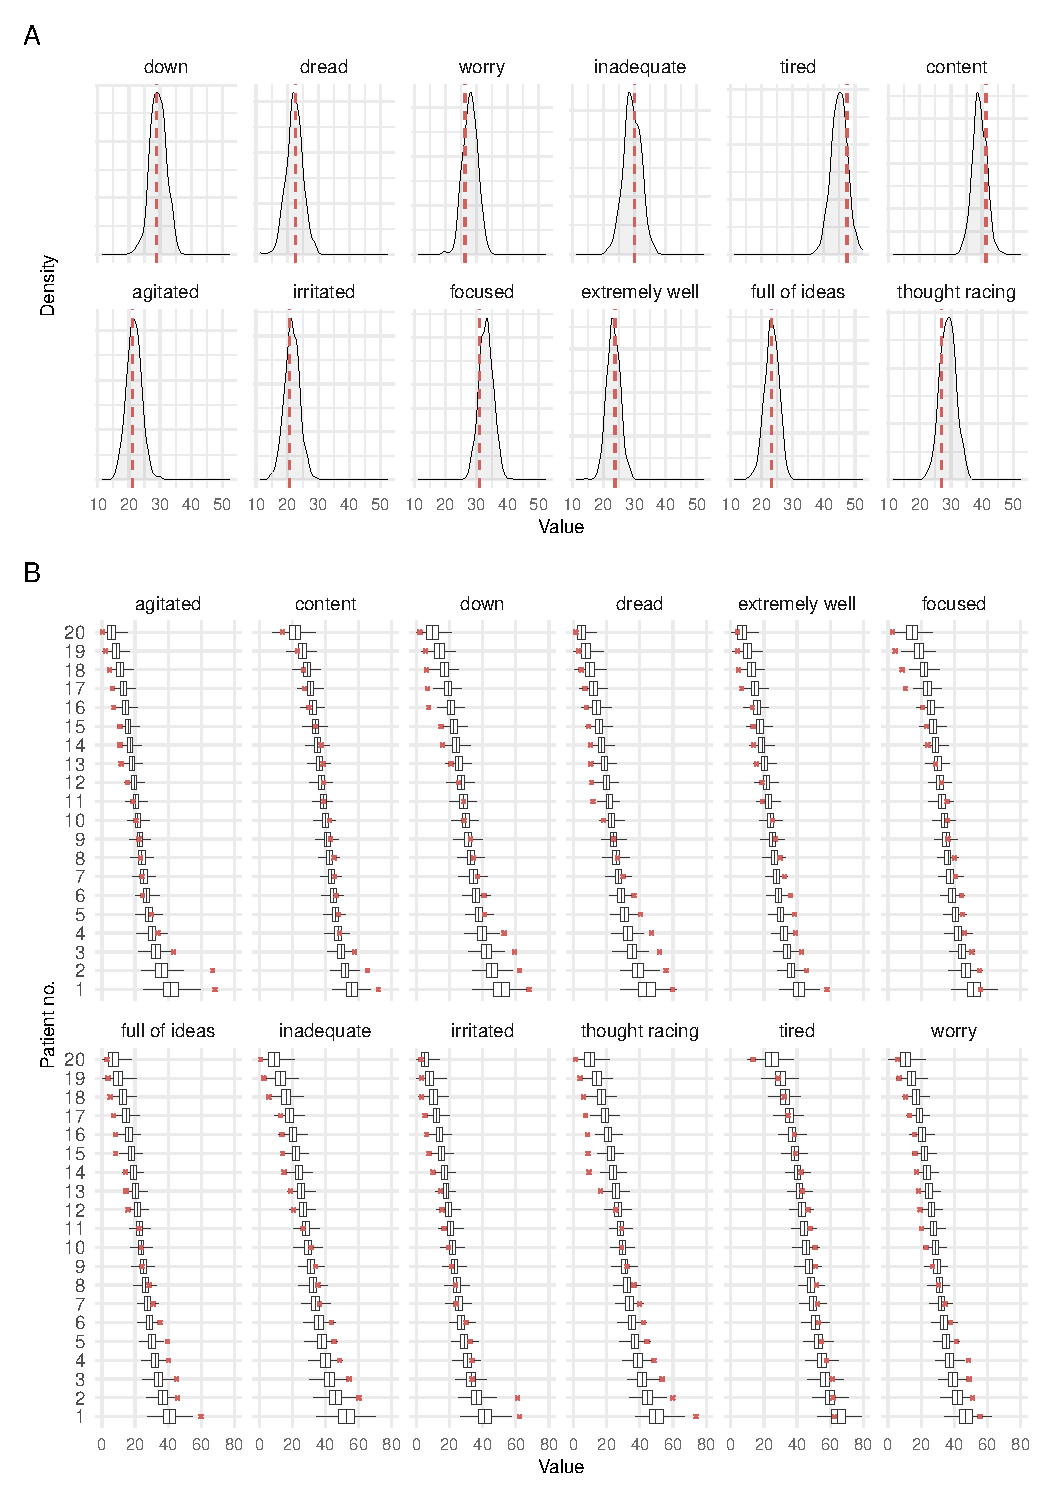
\includegraphics[width=0.7\textwidth]{graphics/ppc_mean_emiss.pdf}
\flushleft
\footnotesize
\justifying
 Panel A represent the group-level emission distribution scores on considered items observed in the data (red dashed line) and the distribution of scores multiply sampled from the MEDHMM (shaded grey distributions). Panel B represent the subject-level emission distribution mean scores on considered items observed in the data (red crosses) and the distribution of scores multiply sampled from the MEDHMM (boxplots).\label{ppc_out_mean_medhmm}
\end{figure}

\begin{figure}[h]
\centering
\caption{Empirical example: Posterior predictive checks (PPCs) for MHMM}
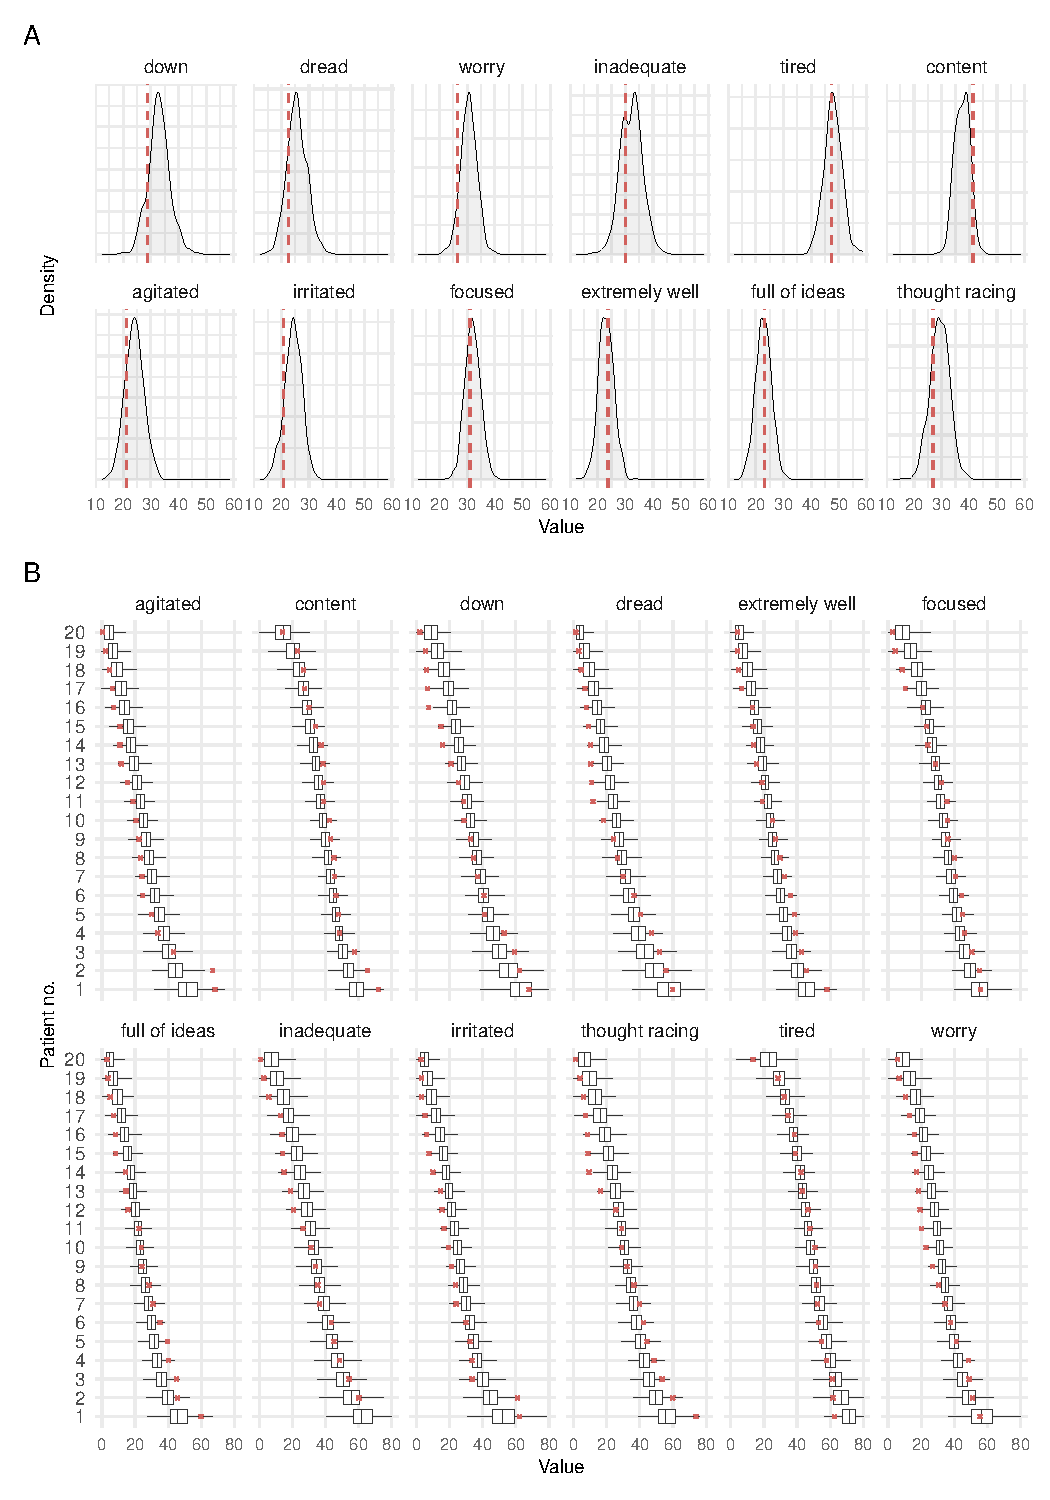
\includegraphics[width=0.8\textwidth]{graphics/ppc_mean_hmm.pdf}
\flushleft
\footnotesize
\justifying
 Panel A represent the group-level emission distribution scores on considered items observed in the data (red dashed line) and the distribution of scores multiply sampled from the MHMM (shaded grey distributions). Panel B represent the subject-level emission distribution of mean scores on considered items observed in the data (red crosses) and the distribution of scores multiply sampled from the MEDHMM (boxplots). 
 \label{ppc_out_mean_mhmm}
\end{figure}


\begin{figure}[h]
\caption{Empirical example: The group-level MHMM transition probability matrix}
    \centering
    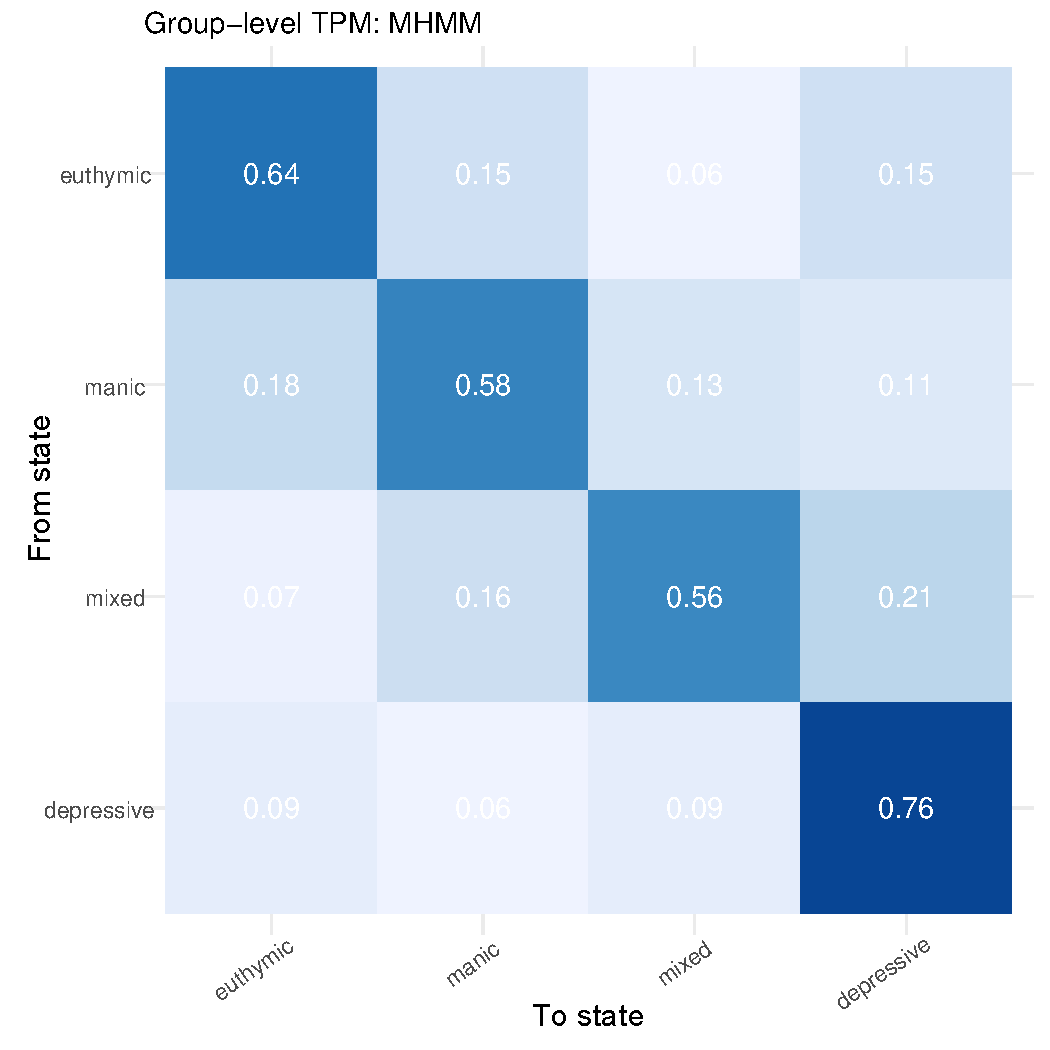
\includegraphics[width=0.65\linewidth]{graphics/group_trandition_matricesvv2.pdf}
    \label{emp_group_trans}
\end{figure}